\chapter{TuMag's design and calibration.}

In this chapter we take the first steps of the journey of developing an instrument to observe the Sun. We will define... 

The SUNRISE III mission aims to study and stablish the relations and couplings between the phenomena ocurring at different layers of the Sun's surface. With this purpose in mind, three different post-focal instruments were included in the design, each of them responsible of observing at different regions of the spectrum. The SUNRISE UV Spectropolarimeter and Imager (SUSI, \textbf{REFERENCIA}), which will observe the spectra between 309 nm and 417 nm; The Sunrise Chromospheric Infrared spectroPolarimeter (SCIP, \textbf{REFERENCIA}), which will observe the near-infrared; and lastly, the Tunable Magnetograph (TuMag), which will observe three spectral lines in the visible, at 525.02 nm, 525.06 nm and 517 nm. 

The design from scratch of an instrument such as this is very complex. There are many things that have to be meticulously designed and tested which span many fields of expertise, like optics, electronics, software, hardware, or thermal design. To avoid undue extension of this thesis, we will focus on the aspects of the design directly related to the \textbf{TO QUE}, that is, regarding the spectral, imaging and polarimetric capabilities of the instrument. 

\section{A brief introduction to spectropolarimeters.}

Spectropolarimeters, as suggested by the name, are devices that measure the spectral and polarimetric properties of light, or in other words, that measure the polarization state of light as a function of wavelength. Their use is widely extended in astrophysics due to the huge amout of information about the light source we can infer from these properties.

In solar physics, it is common to encounter two distinct types of spectropolarimeters, distinguished by their approach to spectroscopy: slit-based spectrographs, such as SUSI and SCIP, and narrow-band tunable filtergraphs, like TuMag. The latter preserve spatial resolution by capturing two-dimensional images of the solar scene at the expense of sacrificing spectral resolution. Conversely, slit-based spectrographs provide excellent spectral resolution but have a limited spatial resolution. 

Regardless of how spectroscopy is carried out, spectropolarimeters must be able to measure the polarization state of light. That is, they must be capable of determining the Stokes parameters  of the incident light. These four parameters, usually grouped in a pseudo-vector: $[I, Q, U, V]$, were defined by Stokes in \cite{Stokes_vector} as a mathematical formalism to completely define to polarization state of light. The first parameter, $I$, represents the total intensity; $Q$ and $U$ provide information about the intensity of linearly-polarized light, at 0º and 90º, respectively; and lastly, $V$, accounts for the intensity of circularly polarized light. 

Excellent polarimetric sensitivity and spectral resolution are wasted if the optical capabilities of the instrument are not up to par. The design of these instruments must achieve diffraction-limited imaging, with a signal-to-noise ratio ensuring a polarimetric sensitivity of 1000 (typically), and the best spatial resolution the telescope allows, all without sacrificing spectral resolution and accomplishing this in the shortest possible time.

When designing the instrument, one must balance these three properties: spectral, optical, and polarimetric capabilities, trying to improve the performance in all of them without sacrificing too much. In the following sections, we will delve into each of these aspects in more detail.

\subsection{Spectroscopy}

Narrow-band tunable spectrographs play a significant role in this thesis. They will be extensively discussed in this chapter, particularly in relation to the design and calibration of TuMag, and again in Chapters \ref{CH:Pipeline} and \ref{CH:challenges} when addressing TuMag's pipeline and the correction of data produced by these instruments. Therefore, for the sake of simplicity, we will focus exclusively on this type of spectrographs from this point onward.

\textcolor{red}{CAMBIAR ESTO}.

Fabry-Pérot Interferometers (FPIs), also known as etalons (used interchangeably), represent one of the most prevalent forms of narrow-band tunable spectrographs. Composed by a resonant optical cavity formed by two distinct optical media, these devices allow only the passage of light with wavelengths corresponding to constructive interference within the cavity. 

The transmission profile of an etalon, being produced by an interference phenomenon, is characterized by a series of narrow and periodic transmission peaks. The wavelengths at which this resonance peaks are located, their width, and their separation are determined solely by the physical properties of the etalon. In fact, it is not difficult to demonstrate \citep{franI} that a resonant cavity produces a periodic transmission profile, with maxima occurring at a wavelength $\lambda$ such that:

\textcolor{red}{REVISAR -> VÁLIDO PARA TELECENTRIC??} 

\begin{equation}
\lambda = \frac{2nd\cos \theta}{m}\ ,
\label{eq_ch2: order_sorting}
\end{equation}
where $n$ is the refractive index of the medium inside the cavity, $d$ is the distance between the mirrors, $\theta$ is the angle of incidence of the incoming light ray and m is the interferential order ($m \in \mathbb{Z} $). 

With Eq.~\eqref{eq_ch2: order_sorting} in mind, it is clear that an etalon allows for tuning the wavelengths of the transmission peaks by either changing the distance between the mirrors or by altering the refractive index. Although changing the angle of incidence also results in a wavelength shift, it introduces other issues, such as ghost images or profile broadening in telecentric configurations, among other effects. Consequently, the angle is not used for wavelength tuning.

To tune to a single wavelength (or a very narrow band around it), it is necessary to isolate one transmission peak (main order). This is typically achieved by using a pre-filter that only allows light with wavelengths near the desired measurement region to pass through. This ensures that no light reaches the etalon that could pass through it due to interference orders other than the main one (secondary orders). 

\begin{figure}
  \centering
  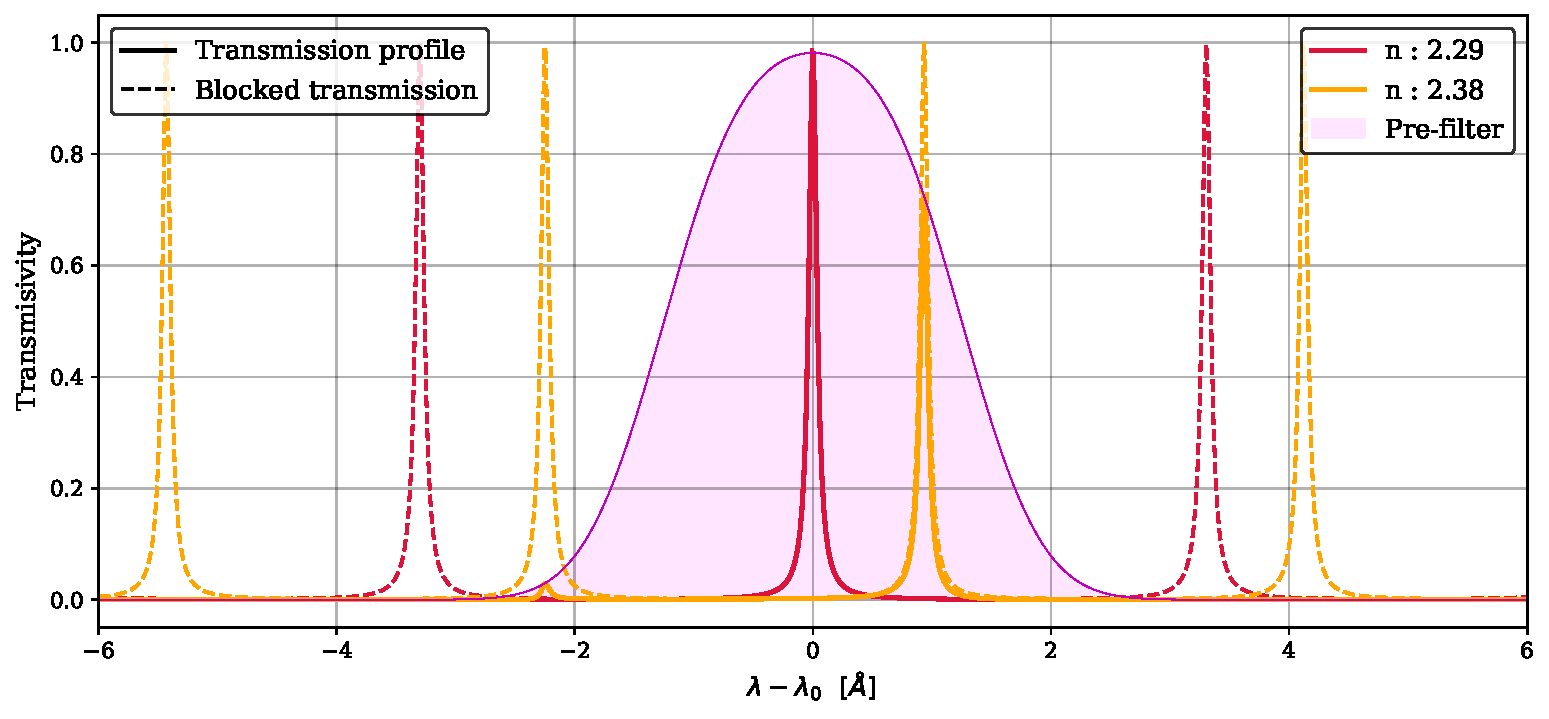
\includegraphics[width = \textwidth]{figures/Introduction_to_spectropolarimeters/Etalon_and_prefilter_example.pdf}
  \caption{Transmission profiles of the same etalon with varying refractive indices (n). The dashed lines represent the original transmission profile, while the solid lines indicate the portion of the transmission profile that passes through the order-sorting pre-filter (shaded purple area).} 
  \label{fig_ch2: etalon_example}
\end{figure}

Figure \ref{fig_ch2: etalon_example} shows a simulation of the spectral behavior of this optical setup. The order-sorting pre-filter is shown with a shaded purple area and the unaltered transmission profile of the etalon is shown in dahsed lines for different values of the refractive index. In solid lines, the resulting transmission profile is shown, that is, the transmission allowed through both the pre-filter and etalon at the same time. 

In reality, the spectral and optical properties of FPIs can be quite complex and are influenced not only by their physical characteristics but also by their optical configuration, whether collimated or telecentric. In Chapter 2, we provide a detailed overview of the properties of each configuration, their differences, and the challenges involved in using these devices for data correction.

\subsection{\label{susec_spectropolarimeters: Imaging}Imaging}

Aquí que va? PSFs Phase diversity? 


\subsection{Polarimetry}

\textcolor{red}{As previously noted, determining the polarization state of light requires the determination of the components of the Stokes vector. However, these parameters cannot be measured directly since we only know how to measure intensities. Since they are  Thus, measuring the polarization of light always involves multiple measurements at once. Specifically, a number equal to the number of elements to be determineed: four for the complete Stokes vector, or two, if only the circular polarization and total intensity are to be measured. This is the root of the difficulties in measuring polarization, as the need for multiple measurements makes them much more susceptible to spurious effects compared to individual measurements.} Cambiar que es un jaleo. 

Mathematically, the effect on polarization of a linear and finite system can be treated as a combination of linear transformations on the Stokes vector and, therefore, can be represented by a matrix in $\mathbb{R}^4$, known as the \textit{Mueller Matrix}. Let $\textbf{M}$ be the matrix that describes these transformations, then the polarization state that reaches the detector follows:

\begin{equation}
  \textbf{I}_{out} = \textbf{M}\textbf{I}_{in},
\end{equation}
where $\textbf{I}_{in}$ and $\textbf{I}_{out}$ are the Stokes vectors of the light that reaches the instrument, and the detector, respectively. However, since we only know how to measure intensities, the actual quantity measured by our CCD is: 

\begin{equation}
  I_{obs} = m_{00}I_{in} + m_{01}Q_{in} + m_{02}U_{in} + m_{03}V_{in} \ \ ,
\end{equation}
where $m_{0i}$ is the i-th element of the first row of the Mueller Matrix. This means that the intensity we measure is a linear combination of the different polarization states of the incoming light. To determine the values of the individual parameters $I_{in}$, $Q_{in}$, $U_{in}$, and $V_{in}$, further independent measurements are necessary, which can be achieved by modifying the Mueller matrix. In particular, it is easy to see that four independent measurements are required in order to construct a system of equations that allows us to determine the full Stokes vector. This process is known as modulation, and the four independent measurements are referred to as modulations.

If we denote each of the modulations by $I _ j$ with $j \in \left\{ 1, 2, 3, 4\right\}$, we can construct the following system of equations:

\begin{equation}
  \begin{pmatrix}
  I _ 1 \\
  I _ 2 \\
  I _ 3 \\
  I _ 4
  \end{pmatrix} = 
  \underbrace{\begin{pmatrix} 
      m ^ 1 _ {01} & m ^ 1 _ {02} & m ^ 1 _ {03} & m ^ 1 _ {04} \\ 
      m ^ 2 _ {01} & m ^ 2 _ {02} & m ^ 2 _ {03} & m ^ 2 _ {04} \\
      m ^ 3 _ {01} & m ^ 3 _ {02} & m ^ 3 _ {03} & m ^ 3 _ {04} \\
      m ^ 4 _ {01} & m ^ 4 _ {02} & m ^ 4 _ {03} & m ^ 4 _ {04} 
  \end{pmatrix}}_ {\textbf{O}}
  \begin{pmatrix}
    I _ {in} \\
    U _ {in} \\
    Q _ {in} \\
    V _ {in}
    \end{pmatrix} \, 
\end{equation}
where the superindex in $m ^j _{oi}$ denotes the values of the Mueller Matrix for each modulation. Through straightforward algebra, it is easy to see that the stokes vector of the incoming light can be determined by $\textbf{I}_{in} = \textbf{D}\textbf{I}_{obs}$, where $\textbf{D}$ is the demodulation matrix, the inverse of the modulation matrix, $\textbf{O}$, and $\textbf{I}_{obs}$ is the vector containing the 4 measured modulations. Accurately determining $\textbf{O}$ during the instrument calibration process is crucial, as the determination of the Stokes components depends entirely upon it.

 
\subsection{What for? Zeeman effect.}





\section{The Tunable magnetograph: TuMag}

TuMag is a wavelength-tunable spectropolarimeter capable of probing the line-of-sight velocity ($v$los) and the vector magnetic field ($\vec{B}$) in the photosphere and the low chromosphere. This means that TuMag must be able to switch between different spectral lines and measure the full stokes vector at each observed wavelength. 

TuMag's design and properties are a direct consequence of the scientific purpose for which it has been conceived and its requirements. 

\subsection{Optical design and image quality.}



\subsection{Spectral capabilities}

As a spectrograph, TuMag is able to tune the wavelength of the measurements through a Fabry-Pérot interferometer (FPI), and select between three different spectral lines through the different pre-filters located on the filter wheel. 

The FPI, or etalon, is a LiNbO$_3$-based ...



\subsection{Polarimetric capabilities}



\section{Calibration of TuMag}